
% normal

\newcommand{\varDUCC}{\text{DUCC}}
\newcommand{\varOS}{\text{OS}}
\newcommand{\varJava}{\text{Java}}
\newcommand{\varJVM}{\text{JVM}}
\newcommand{\varLinux}{\text{Linux}}
\newcommand{\varSpring}{\text{Spring}}
\newcommand{\varUIMA}{\text{UIMA}}
\newcommand{\varUnstructuredInformationManagementArchitecture}{\text{Unstructured Information Management Architecture}}
\newcommand{\varUIMAAS}{\text{UIMA-AS}}
\newcommand{\varUIMACore}{\text{UIMA-Core}}
\newcommand{\varUIMAAsynchronousScaleout}{\text{UIMA Asynchronous Scaleout}}

\newcommand{\varLinuxControlGroup}{\text{Linux Control Group}}
\newcommand{\varLinuxControlGroups}{\text{Linux Control Groups}}

\newcommand{\varDistributedUIMAClusterComputing}{\text{Distributed \varUIMA~Cluster Computing}}

\newcommand{\varOrchestrator}{\text{Orchestrator}}
\newcommand{\varResourceManager}{\text{Resource Manager}}
\newcommand{\varServicesManager}{\text{Services Manager}}
\newcommand{\varProcessManager}{\text{Process Manager}}
\newcommand{\varAgent}{\text{Agent}}
\newcommand{\varAgents}{\text{Agents}}
\newcommand{\varJobDriver}{\text{JobDriver}}
\newcommand{\varWebServer}{\text{WebServer}}
\newcommand{\varWebServerInterface}{\text{WebServer Interface}}
\newcommand{\varCommandLineInterface}{\text{Command Line Interface}}
\newcommand{\varApplicationProgramInterface}{\text{Application Program Interface}}

\newcommand{\varScheduler}{\text{Scheduler}}

\newcommand{\varOR}{\text{OR}}
\newcommand{\varRM}{\text{RM}}
\newcommand{\varSM}{\text{SM}}
\newcommand{\varPM}{\text{PM}}
\newcommand{\varJD}{\text{JD}}
\newcommand{\varWS}{\text{WS}}
\newcommand{\varCLI}{\text{CLI}}
\newcommand{\varAPI}{\text{API}}

\newcommand{\varActiveMQ}{\text{ActiveMQ}}
\newcommand{\varCamel}{\text{Camel}}
\newcommand{\varJetty}{\text{Jetty}}
\newcommand{\varjQuery}{\text{jQuery}}
\newcommand{\varLogger}{\text{Log4J}}

\newcommand{\varApacheActiveMQ}{\text{Apache Active MQ}}
\newcommand{\varIBMWebSphereMQ}{\text{IBM WebSphere MQ}}

\newcommand{\varNetworkFileSystem}{\text{Network File System}}
\newcommand{\varNFS}{\text{NFS}}

\newcommand{\varHadoopDistributedFileSystem}{\text{Hadoop Distributed File System}}
\newcommand{\varHDFS}{\text{HDFS}}

\newcommand{\varNodeMachineComputer}{\text{node (machine, computer)}}
\newcommand{\varNodesMachinesComputers}{\text{nodes (machines, computers)}}

\newcommand{\varJob}{\text{Job}}
\newcommand{\varJobs}{\text{Jobs}}
\newcommand{\varReservation}{\text{Reservation}}
\newcommand{\varReservations}{\text{Reservations}}
\newcommand{\varService}{\text{Service}}
\newcommand{\varServices}{\text{Services}}

\newcommand{\varManagedReservations}{\text{Managed Reservations}}
\newcommand{\varUnmanagedReservations}{\text{Unmanaged Reservations}}

\newcommand{\varPingOnly}{\text{Ping-Only}}

\newcommand{\varGB}{\text{GB}}
\newcommand{\varUser}{\text{user}}

\newcommand{\varPipeline}{\text{pipeline}}

% typewriter

\newcommand{\varCompleted}{\texttt{Completed}}
\newcommand{\varReceived}{\texttt{Received}}

\newcommand{\varController}{\texttt{Controller}}

\newcommand{\varORmap}{\texttt{OR-map}}

\newcommand{\varProcessThreadCount}{\texttt{process\_thread\_count}}
\newcommand{\varNumberOfInstances}{\texttt{number\_of\_instances}}
\newcommand{\varSchedulingClass}{\texttt{scheduling\_class}}

\newcommand{\varDuccAdministrators}{\texttt{ducc.administrators}}
\newcommand{\varDuccProperties}{\texttt{ducc.properties}}

\newcommand{\varPID}{\texttt{PID}}

\newcommand{\varINFO}{\texttt{INFO}}
\newcommand{\varDEBUG}{\texttt{DEBUG}}
\newcommand{\varTRACE}{\texttt{TRACE}}

\newcommand{\varIScheduler}{\texttt{IScheduler}}

\newcommand{\varRogue}{\texttt{Rogue}}

\newcommand{\varDuccling}{\texttt{ducc\_ling}}

% italics

\newcommand{\varNull}{\textit{null}}

\newcommand{\varShares}{\textit{DUCC-Shares}}
\newcommand{\varShare}{\textit{DUCC-Share}}

\newcommand{\varJdShares}{\textit{JD-Shares}}
\newcommand{\varJdShare}{\textit{JD-Share}}

\newcommand{\varSendAndReceiveCAS}{\textit{UIMA-AS sendAndReceiveCAS}}

\newcommand{\varCAS}{\textit{CAS}}
\newcommand{\varCASes}{\textit{CASes}}

\newcommand{\varWorkItem}{\textit{WorkItem}}
\newcommand{\varWorkItems}{\textit{WorkItems}}

\newcommand{\varPendingQueued}{\textit{PendingQueued}}
\newcommand{\varPendingAssigned}{\textit{PendingAssigned}}
\newcommand{\varNotPending}{\textit{NotPending}}

\newcommand{\varAlienDetected}{\texttt{alien detected}}

% uima

\newcommand{\varCollectionReader}{\textit{Collection Reader}}
\newcommand{\varCR}{\text{CR}}
\newcommand{\varAnalysisEngine}{\textit{Analysis Engine}}
\newcommand{\varAE}{\text{AE}}
\newcommand{\varJobProcess}{\textit{Job Process}}
\newcommand{\varJP}{\text{JP}}

% body

\chapter{Platform}

    The \varDistributedUIMAClusterComputing~(\varDUCC) platform comprises software 
    designed to facilitate the scale-out of 
    \varUnstructuredInformationManagementArchitecture~(\varUIMA) pipelines on a 
    collection of \varNodesMachinesComputers~shared "fairly" by a group of users.
    
    The major components of \varDUCC~are the \varOrchestrator~(\varOR), the \varJobDriver~(\varJD), 
    the \varResourceManager~(\varRM), the \varProcessManager~(\varPM), the \varServicesManager~(\varSM), 
    the \varAgents, the \varCommandLineInterface~(\varCLI), the \varApplicationProgramInterface~(\varAPI), 
    and the \varWebServer~(\varWS).
        
    \section{Highlights}
    
    \varDUCC~was conceived to address the following:
    
    \begin{itemize}
      \item manage a cluster of machines for \varUIMA~workloads
      \item highly configurable "fair-share" resource allocation system
      \item application code runs with credentials of submitting user
      \item "virtual machine" resources for user processes allocated instantaneously via \varLinuxControlGroups
      \item extensive Web, \varCLI~and \varAPI~interfaces
      \item rich debugging support for user processes
    \end{itemize} 
    
    \section{Architecture}
    
    The \varDUCC~platform employs building-block software from the open-source community
    where possible to achieve it goals. Foremost and not surprisingly \varDUCC~employs in
    its foundation \varUIMAAS, which in-turn relies upon \varUIMA-Core.
    
    Additionally, \varCamel~is used for inter-component communications.
    \varActiveMQ~is employed to process work items amongst a distributed set of work item processors.
    Logging is facilitated by \varLogger. \varJetty~is used for the \varWebServer~and \varjQuery~is deployed
    to web browsers.  And various other open-source softwares are likewise employed.
    
    By employing reliable open-source code where possible, the amount of custom code needed
    to develop and maintain \varDUCC~functionality is minimized. And substitution of implementation
    for equivalent functionality is possible, for example replacing \varApacheActiveMQ~with 
    \varIBMWebSphereMQ.
    
    \begin{figure}[h]
    \centering
    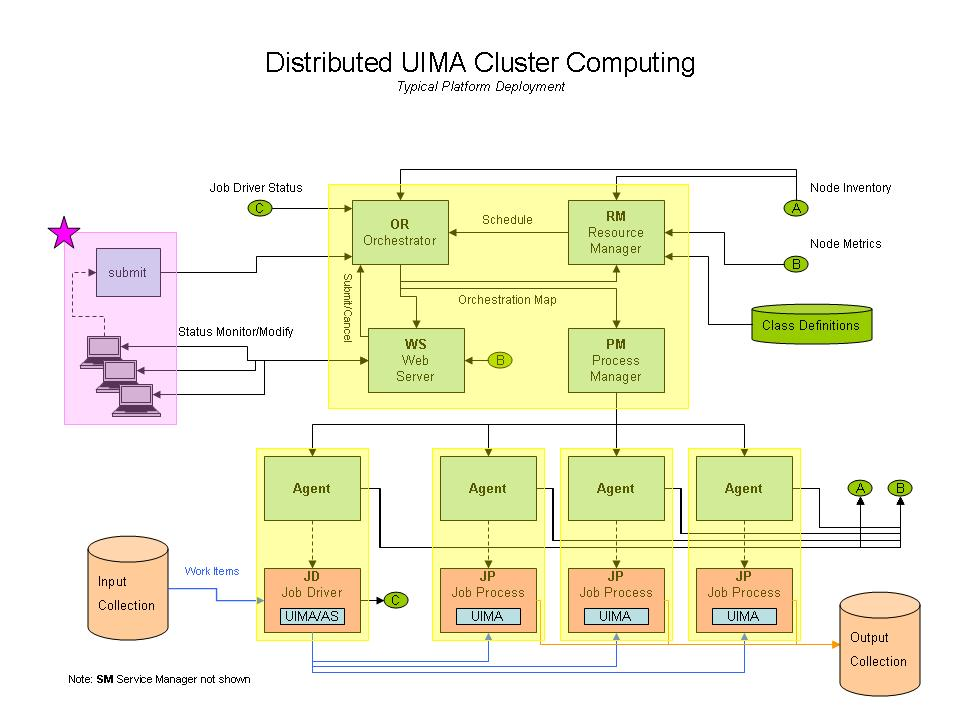
\includegraphics[width=6.5in]{images/ducc-arch.jpg}
    \caption{\varDUCC~Architecture}
    \label{fig:\varDUCC~Architecture}
    \end{figure}

    \section{\varJobs}

    The main focus of the system is running "batch" \varJobs~comprising \varUIMA~pipelines.
    
    Users submit \varJobs~to the system to be deployed and executed. \varJobs~have a
    life-cycle from birth to death during which time a (normally) finite collection of
    work items are processed by one or more \varUIMA~pipelines. \varJobs~consist of two
    parts: a singleton work item supplier, known in \varUIMA~parlance as a
    \varCollectionReader~(\varCR); and one or more pipelines, each known in \varUIMA~parlance
    as an \varAnalysisEngine~(\varAE).
        
    \subsection{Characteristics}   
    
    \varDUCC~facilitates "fair-share" \varUIMA~pipeline scale-out.
    
    The \varUIMA~pipelines comprising a \varJob~represent "embarrassingly parallel" 
    deployments. Over time, a \varJob~may expand and contract with respect to the number of 
    \varUIMA~pipelines deployed during its lifetime. This may be due to the introduction 
    or completion of other \varJobs, the rise and fall of other resource consumers such 
    as \varReservations~or \varServices, and the addition or removal of computer resources 
    to the cluster.
    
    With respect to contraction, each \varUIMA~pipeline must be prepared to
    process work items that may have been partially processed previously.
   
    Pipelines themselves may comprise one or more duplicate threads, such that each
    pipeline can simultaneously process multiple work items.
    The number of pipelines and threads per pipeline are configurable per \varJob.
   
    \subsection{Performance}  
    
    For the distributed environment, \varDUCC~relies upon a \varNetworkFileSystem~(\varNFS)
    for file access to work items.
    High performance is achieved through \varNFS~data sharing and (via \varActiveMQ) the passing of
    data-handles that are utilized by the "embarrassingly parallel" pipelines.
    
    \section{\varReservations}
    
    To help support Jobs, \varDUCC~provides facilities for \varReservations~of two types: 
    Managed and Unmanaged. \varReservations, once allocated, are preserved until 
    canceled. 
    
    \varManagedReservations~(MRs) comprise "arbitrary" processes, for example Java
    programs, c-programs, bash shells, etc.
    
    \varUnmanagedReservations~(URs) comprise a resource that can be utilized for any 
    purpose, subject to the limitations of the assigned \varShare~or \varShares.
            
    \section{\varServices}
       
    To help support \varJobs, \varDUCC~provides facilities for \varServices~of two types: 
    \varUIMA~and \varPingOnly. \varServices~can be predefined in a registry, and 
    \varJobs~can declare dependency on one or more of them.
    
    \varServices~can be shared by my multiple \varJobs~or can be tied to just one.
    \varServices~can be started at \varDUCC-boot time or at \varService-definition time or
    at \varJob~launch time.
    
    \varServices~can be expanded and contracted by command or on-demand.  
    \varServices~can be stopped by command or due to absence of demand.
    
    \varServices~nominally exists for reasons of efficiency due to high start-up costs
    or high resource consumption.  Benefits of cost amortization are realized by sharing
    \varServices~amongst a collection of \varJobs~rather than employing a private copy 
    for each.
    
    The lifecycle of each \varUIMA~\varService~is managed by \varDUCC, which is not the
    case for \varPingOnly~\varServices.  However, each comprises a "pinger" which 
    adheres to a standard interface and provides health and statistical information.
    
    \section{Management} 
    
    The \varDUCC~system employs several management techniques to fairly apportion
    resources.
    
    \subsection{Memory Shares} 
    
    The \varDUCC~system partitions the entire set of available resources comprising
    \varNodesMachinesComputers~into \varShares.
    
    Partitioning of the available \varNodesMachinesComputers~into \varShares~facilitates
    multitenancy amongst a collection of \varDUCC-managed user applications consisting 
    of \varUIMA~pipelines.
    
    One or more \varShares~are allocated and sub-partitioned into \varJdShares.
    
    Users submit \varJobs~to the \varDUCC~system specifying a requisite memory size.
    Each \varJob~is allocated one \varJdShare~and, based upon user specified
    memory size, one or more \varShares. 
    Likewise, users submit \varReservations~and \varServices~also comprising memory size
    information.  These are assigned \varShares~only.
    
    New \varJobs, \varReservations~and \varServices~may only enter the system when
    there are sufficient unallocated \varShares~available. To make room for newly arriving
    submissions, the \varResourceManager~may preempt use of already previously
    assigned \varShares~for re-assignment.
    
    \subsection{\varLinuxControlGroups} 
    
    If available, \varDUCC~employs \varLinuxControlGroups~to enforce limits on
    deployed applications. Exceeding limits penalizes only the offender.
    For example, if a user application exceeds its memory \varShare~size then it is forced
    to swap while other co-resident applications remain unaffected.
    
    \subsection{Preemption} 
        
    Preemption is employed by \varDUCC~to re-apportion \varShares~when new work is submitted.
    
    For example, presume a simple \varDUCC~system with just one preemptable scheduling class
    and resources comprising 11 \varShares. Further, suppose that 1 \varShare~is allocated 
    for partitioning into \varJdShares.
    When the Job #1 is submitted it is entitled to all remaining 10 shares.  
    When Job #2 arrives, each job is entitled to only 5 shares.
    Thus, 5 \varShares~from Job #1 are preempted and reassigned to Job #2.
    
\chapter{System Organization}

    \section{Single System Image}
    
    \varDUCC~runs on \varLinux. It can be run on a single system in simulation-mode
    or on a cluster (two or more machines). For clusters, \varDUCC~replies upon 
    these requirements:
    
    \begin{itemize}
      \item common userids across the cluster
      
      Each userid must have the same definition on all machines participating
      in the \varDUCC~cluster.
      
      \item a shared filesystem for user and \varDUCC~data across the cluster
      
      Each machine shares a filesystem (commonly provided by NFS) with all 
      machines participating in the \varDUCC~cluster.
      
    \end{itemize} 
    
    \section{Communications}
    
    \varDUCC~comprises a collection of singleton and distributed daemons that need
    to coordinate activities.  This coordination is accomplished via messaging.
    
    The system is fault tolerant with respect to lost messages, since
    publications occur at regular intervals and each message encapsulates
    the current and/or desired state for the target audience.
    As such, actions may be be delayed but will be carried out as soon as the
    next message arrives.
    
    \section{Daemons}
    
    \varDUCC~is implemented through a collection of configurable singleton 
    and distributed daemons.
    
    \subsection{\varOrchestrator~(\varOR)} 
    
    There is one \varOrchestrator~per \varDUCC~cluster.
    
    The duties of the \varOrchestrator~are:
    \textit{
      % 
% Licensed to the Apache Software Foundation (ASF) under one
% or more contributor license agreements.  See the NOTICE file
% distributed with this work for additional information
% regarding copyright ownership.  The ASF licenses this file
% to you under the Apache License, Version 2.0 (the
% "License"); you may not use this file except in compliance
% with the License.  You may obtain a copy of the License at
% 
%   http://www.apache.org/licenses/LICENSE-2.0
% 
% Unless required by applicable law or agreed to in writing,
% software distributed under the License is distributed on an
% "AS IS" BASIS, WITHOUT WARRANTIES OR CONDITIONS OF ANY
% KIND, either express or implied.  See the License for the
% specific language governing permissions and limitations
% under the License.
% 
\begin{description}
  \item receive and act upon user submitted application requests;
  \item manage and publish common state to a set of distributed components;
  \item maintain checkpoint and historical state;
  \item manage the lifecycle of jobs, services, and reservations.
\end{description}
    }
    
    The \varOrchestrator~provides essential functionality for operation of the
    \varDUCC~system.
    It is configurable and tunable.
    
    The \varOrchestrator~receives user requests to start, stop and modify 
    Jobs, Services and Reservations. It manages the life-cycles of these
    entities, each deployed to a managed cluster of machines 
    (nodes, computers).
    
    The \varOrchestrator~both publishes and receive reports.  
    The \varOrchestrator~publication is also known as the \varORmap, which is
    the final authority on the state of Jobs, Reservations, and Services.
    All other \varDUCC~components respect the state published by the 
    \varOrchestrator~and each carries out its assigned duties accordingly.
    
    \subsubsection{Controller} 
    \label{Controller}
    
    The \varOrchestrator~Controller responsibilities entail receiving user 
    submitted requests and processing them to completion in accordance with 
    an instance of the appropriate state machine. 
    
    User submitted requests comprise:
    
    \begin{itemize}
      \item Job \{ Start, Stop, Modify \}
      \item Reservation \{ Start, Stop, Modify \}
      \item Service \{ Start, Stop, Modify \}
      \item Individual Process \{ Stop \}
    \end{itemize} 
    
    The Controller responsibilities further entail receiving status messages
    from other \varDUCC~components and advancing the state machines of user 
    submitted Jobs, Reservations, and Services as necessary. 
    
    Additionally and importantly, the Controller is the final authority
    for the \varDUCC~system state comprising active Jobs, Reservations, and 
    Services. The Controller publishes \varDUCC~system state at regular intervals
    for consumption and use by all other \varDUCC~components.
    
    \subsubsection{Authenticator} 
    
    The authenticator determines whether or not the requesting user is a
    \varDUCC~administrator. Such users have special privileges, such as:
    
    \begin{itemize}
      \item the ability to control \varDUCC~system functions
      \item the ability to act on behalf of other users
    \end{itemize}     
    
    The file \varDuccAdministrators~comprises the list of privileged \varDUCC~users.
    
    \subsubsection{Validation} 
    
    Each request to submit, cancel or modify is validated against a set of
    criteria that define acceptableness. In the case of missing information,
    a default value may be employed.
    
    Presently, the following keys are validated by the \varOrchestrator:
    
    \begin{itemize}
      \item \varProcessThreadCount
      \item \varNumberOfInstances
      \item \varSchedulingClass
    \end{itemize} 
    
    Other keys are validated by the \varCommandLineInterface, prior to arrival
    at the \varOrchestrator.
    
    \subsubsection{Factory} 
    
    Once accepted, submit requests proceed through a corresponding factory
    to have a state machine representation entered into the published
    \varORmap~with initial state of \varReceived.  The request remains 
    active until it advances to final state \varCompleted.
    
    Each factory-created representation comprises appropriate information as follows:
    
    \begin{itemize}
    
      \begin{itemize}
      \item standard information
        \begin{itemize}
          \item unique identifier (assigned by \varDUCC)
          \item type {Job, Reservation, Service}
          \item user name
          \item submitting \varPID
          \item date of submission
          \item date of completion (initially \varNull)
          \item description (text supplied by user)
        \end{itemize} 
      \item scheduling information
        \begin{itemize}
          \item scheduling class
          \item scheduling priority
          \item scheduling max shares
          \item scheduling min shares
          \item scheduling threads per share
          \item scheduling memory size
          \item scheduling memory units
        \end{itemize} 
      \item job driver information
        \begin{itemize}
          \item java command
          \item java classpath
          \item environment variables
          \item user log directory
          \item MQ broker
          \item MQ queue
          \item \varCollectionReader~descriptor
          \item \varCollectionReader~overrides
          \item getMeta timeout value
          \item work item processing timeout value
          \item work item processing exception handler
          \item node identity
          \item \varLinuxControlGroup~limits
          \item state
        \end{itemize} 
      \item job process information (one or more instances)
        \begin{itemize}
          \item java command
          \item java classpath
          \item environment variables
          \item user log directory
          \item MQ broker
          \item MQ queue
          \item deployment descriptor or aggregate data
          \item initialization failure limits
          \item node identity
          \item \varLinuxControlGroup~limits
          \item state
          \item service dependencies
        \end{itemize} 
      \item service information (one or more instances)
        \begin{itemize}
          \item See job process information above.
        \end{itemize} 
      \item managed reservation information
        TBD      
      \item unmanaged reservation information
        TBD          
    \end{itemize} 
    
    \subsubsection{Checkpoint Supervisor} 
    
    The Checkpoint Supervisor provides functions to save and restore state information
    to/from persistent storage. State is stored whenever a significant change occurs.
    State is restored at \varOrchestrator~boot time.
    
    Saving and restoration of state facilitates reasonable continuity of service
    between \varOrchestrator~lifetimes.
    
    \subsubsection{State Supervisor} 

    The State Supervisor receives and examines publications from other
    \varDUCC~components, records and distributes pertinent information obtained
    or derived, and advances state machines appropriately.
    
    Publications are received from these components:
    
    \begin{itemize}
    
    \item Job Driver(s)
    \item Resource Manager
    \item Services Manager
    \item Agent(s) Inventory
      
    \end{itemize} 
    
    Information from these sources is recorded in the \varORmap. 
    Based on information derived from all sources, the 
    \varOrchestrator~advances the state machines of currently active 
    entities (Jobs, Reservations, Services). 
    Once the \varCompleted~state is reached, the
    entity is no longer active on the cluster.
    
    Note that \varORmap~is, in-turn, published at regular intervals 
    for use by the other \varDUCC~singleton and distributed components.
    The \varORmap~is the "final authority" on the state of
    each Job, Reservation and Service currently or formerly deployed.
    See \ref{Controller} \varController.
    
    \subsubsection{State Accounting Supervisor} 
        
    The State Accounting Supervisor manages finite state machine for 
    Jobs, Services, and Reservations. It provides functions to:
    
    \begin{description}
    
    \item Advance from the current state to a next valid state
    \item Advance from the current state immediately to the \varCompleted~state
          
    \end{description} 
    
    \subsubsection{\varLinuxControlGroup~Supervisor}  
    
    The \varLinuxControlGroup~Supervisor assigns a maximum size (in bytes) and a composite
    unique identity to each \varShare. This information is published for use
    by Agents to enforce \varLinuxControlGroup~limitations on storage used by the corresponding
    running entity (for example, \varUIMA~pipeline).
    
    Employing \varLinuxControlGroups~ is analogous to defining virtual machines of a certain
    size such that exceeding limits causes only the offending process to suffer
    any performance penalties, while other co-located well-behaved processes
    run unaffected.
    
    \subsubsection{Host Supervisor}
    
    The Host Supervisor is responsible for obtaining sufficient resource for
    deploying the Job Drivers for all submitted Jobs. It interacts with the
    Resource Manager to allocate and de-allocate resources for this purpose.
    It assigns a \varJdShare~to each active Job.
    
    A \varJdShare~is a \varLinuxControlGroup~controlled \varShare~of sufficient size into which a Job
    Driver can be deployed.  A \varJdShare~is usually significantly smaller than
    a normal \varShare.
    
    \subsubsection{Logging / As-User} 
    
    The Logging and As-User modules permit the \varOrchestrator~to write logging data into
    a file contained in "user-space", meaning a file into a directory writable 
    by the submitting user, during processing of the submitted entity 
    (Job, Managed Reservation...).
    
    The Logging module also facilitates the recording to persistent storage of noteworthy
    events occurring during the \varOrchestrator~lifetime. Noteworthiness is configurable
    as various levels, such as \varINFO, \varDEBUG~and \varTRACE.
        
    \subsubsection{Administrators} 
    
    The Administrators module grants users defined in the \varDuccAdministrators~file
    special privileges, such a being able cancel to any user's Job.
    
    \subsubsection{Maintenance} 
    
    The maintenance thread wakes-up at regular intervals to perform the following
    tasks:
    
    \begin{description}
    
      \item Health
      
      The \varOrchestrator~automatically caps Jobs and Services that exceed initialization
      error thresholds, and cancels those that exceed processing error thresholds.
      
      \item MQ Reaper
      
      The \varOrchestrator~cleans-up unused \varJobDriver~AMQ permanent queues for Jobs that have completed.
      
      \item Publication Pruning
      
      The \varOrchestrator~regularly publishes state for all active entities (Jobs, Reservations,
      Services).  It also publishes state for recently completed ones. Pruning removes
      from regular \varOrchestrator~publication completed entities that have been competed past a
      time threshold, nominally one minute.
           
      \item Node Accounting
      
      This module keeps track of each node's state, up or down.  Nodes that do 
      not report for a time exceeding a threshold, typically a few minutes, 
      are considered down. This information is used for Jobs whose Job Driver
      advanced to the \varCompleted~state, whereby corresponding Job Processes on 
      nodes that are reported down are marked as stopped by the \varOrchestrator, as opposed 
      to waiting (potentially forever) for the corresponding Agent to report.
      This prevents Jobs from becoming unnecessarily stuck in the completing
      state.
      
    \end{description} 
    
    \subsection{\varResourceManager~(\varRM, also known as the \varScheduler)}    
        
    There is one \varResourceManager~per \varDUCC~cluster.
    
    The duties of the \varResourceManager~are:
    \textit{
      % 
% Licensed to the Apache Software Foundation (ASF) under one
% or more contributor license agreements.  See the NOTICE file
% distributed with this work for additional information
% regarding copyright ownership.  The ASF licenses this file
% to you under the Apache License, Version 2.0 (the
% "License"); you may not use this file except in compliance
% with the License.  You may obtain a copy of the License at
% 
%   http://www.apache.org/licenses/LICENSE-2.0
% 
% Unless required by applicable law or agreed to in writing,
% software distributed under the License is distributed on an
% "AS IS" BASIS, WITHOUT WARRANTIES OR CONDITIONS OF ANY
% KIND, either express or implied.  See the License for the
% specific language governing permissions and limitations
% under the License.
% 
\begin{description}
  \item fairly allocate constrained resources amongst valid user requests over
  time.
\end{description}
    }
    
    The \varResourceManager~provides essential functionality for operation of the
    \varDUCC~system.
    It is configurable and tunable.
    It is also plug-replaceable.
    
    The \varResourceManager~both publishes and receive reports.  
    The \varResourceManager~receives \varOrchestrator~publications comprising
    Jobs, Reservations, and Services as well as 
    \varAgent~publications comprising inventory and metrics. 
    The \varResourceManager~publication occurs at regular intervals, each
    representing at the time of its publication the desired allocation
    of resources. 
   
    The \varResourceManager~considers various factors to make assignments, including:
    \begin{description}
      \item supply of available nodes;
      \item memory size of each available node;
      \item demand for resource in terms of memory size and class of service comprising Jobs, Reservations and Services;
      \item the most recent previous assignments and desirability for continuity;
    \end{description}
    
    The \varOrchestrator~is the primary consumer of the \varResourceManager~publication
    which it uses to bring the cluster into compliance with the allocation assignments.
    
    The \varResourceManager~adheres to the \varIScheduler~interface. 
    Algorithms adhering to this interface are eligible for replacing
    the \varDUCC~supplied one.
    
    \subsubsection{Job Manager Converter} 
    
    The Job Manager Converter module receives \varOrchestrator~publications and
    updates its internal state with new, changed, and removed map entries
    comprising Jobs, Reservations and Services.
        
    \subsubsection{Node Stability}
    
    The Node Status module evaluates the health of the nodes within the cluster
    for consideration during resource scheduling.  Any node deemed unhealthy is
    removed from the collection of available resources until such time as it
    is once again deemed healthy.
      
    \subsubsection{Node Status} 
        
    The Node Status module receives \varAgent~publications and
    updates its internal state with new, changed, and removed node status entries.
     
    \subsubsection{Resource Manager} 
    
    The \varResourceManager~performs the following:
    
    \begin{description}
      \item receive resource availability reports from \varAgents;
      \item receive resource need requests the \varOrchestrator;
      \item employ a scheduling algorithm at discrete time intervals to:
      \begin{description}
        \item consider the resource supply;
        \item consider the most recent allocation set;
        \item consider new, changed and removed resource demands;
        \item assign a resource to a request;
        \item remove a resource from a request;
        \item publish current allocation set;
      \end{description} 
    \end{description}     
        
    \subsubsection{\varScheduler} 
    
    The \varScheduler~runs at discrete time intervals.
    It assembles information about available nodes in the cluster.
    Each node, based upon its memory size is partitioned into zero or more \varShares.
    Each request (Job, Reservation and Service) is assessed as to the number of
    \varShares~required based upon user-specified memory size. 
    In addition, each request is assessed with respect to the user-specified class-of-service.

    The \varScheduler~considers the most recent previous allocations along with changes
    to supply and demand.  It then produces a new allocation set which the 
    \varResourceManager~publishes as directions to the \varOrchestrator.
    
    \subsection{\varServicesManager~(\varSM)}    
    
    There is one \varServicesManager~per \varDUCC~cluster.
    
    The duties of the \varServicesManager~are:
    \textit{
      \begin{description}
  \item monitor and control processes supporting analytic pipelines distributed over a collection of agent-managed nodes;
\end{description}
    }
        
    The \varServicesManager~provides additional functionality for operation of the
    \varDUCC~system.
    It is configurable and tunable.
    
    Although not essential for the main purpose of the \varDUCC~system, in
    practical terms for large systems the \varServicesManager~is highly 
    desirable for improved resource utilization.
    By using shared services, resources are more effectively employed and
    work items processing is completed sooner.
    
    Some dimensions:
    
    \begin{itemize}
    
      \item long warm-up time
      
      When the service takes a long time to warm-up, the \varJob~in progress
      may have to sit idle for a long time before the first work item can be
      processed until the service upon which it depends has initialized and 
      is ready.
      If the service is already up and ready, this delay can be avoided
      and the \varJob~experiences no service delay.
      
      \item large storage use
      
      When the service has a large memory footprint, it can be far more
      efficient to have multiple \varJobs~share the service rather than
      having separate copies for each.
      
      \item short processing time
      
      Related to large storage use, if the time to process a work item is
      relatively short, again it can be much more efficient to share the
      service amongst multiple \varJobs.
      
      \item not used
      
      If a service has not been used for a relatively long time, it may be 
      better to shut it down and reclaim the resources for use elsewhere, 
      especially on a busy cluster.
            
    \end{itemize}
    
    \subsubsection{Ping Driver} 
    
    This runs the watchdog thread for custom service pingers.
    It ascertains the liveness and healthiness of each service
    known to \varDUCC.
    
    \subsubsection{Service Handler} 
    
    Carries out Service Manager validated request operations.
            
    \subsubsection{Service Manager, API Handler} 
    
    Receives and validates service request operations:
    
    \begin{itemize}
      \item register
      \item unregister
      \item start
      \item stop
      \item query
      \item modify
    \end{itemize}
    
    The \varServicesManager~maintains a registry of services.
    The attributes of these services may include one of more of the following:
    
    \begin{description}
      \item \texttt{permanent}
      A permanent service is one that is kept up so long as the
      \varDUCC~system is running.
      \item \texttt{on-demand}
      An on-demand service is one that is kept up only during the
      lifetime of one or more \varJobs~that declare a dependency on the 
      service
      \item \texttt{lingering}
      A lingering service is one that continues for some limited time
      beyond the lifetime of the last dependent \varJob~in anticipation
      of another \varJob~arrival in the near future.
      \item \texttt{dynamic}
      A dynamic service is one that automatically expands and contracts
      in terms of number of instances to meet demand.
      \item \texttt{registered}
      A registered service is one that is pre-defined, whose definition
      is kept persistently and whose lifecycle is managed by \varDUCC.
      \item \texttt{custom}
      A custom (unregistered) service is one that is not pre-defined, whose definition
      is not kept persistently and whose lifecycle is not managed by \varDUCC.
    \end{description}
  
    The \varServicesManager~keeps within its registry information of
    two types: \texttt{service} and \texttt{meta}.
    
    Type \texttt{service} information includes the following attributes:
    \begin{itemize}
      \item classpath
      \item description
      \item environment
      \item jvm
      \item jvm args
      \item log directory
      \item deployment descriptor
      \item failures limit
      \item memory size
      \item scheduling class
      \item linger time
      \item pinger classpath
      \item pinger log
      \item pinger timeout
      \item service endpoint
      \item working directory
    \end{itemize}
    
    Type \texttt{meta} information includes the following attributes:
    \begin{itemize}
      \item autostart
      \item endpoint
      \item implementors
      \item instances (count)
      \item identifier (number)
      \item ping-active
      \item ping-only
      \item service-active
      \item service-class
      \item service-health
      \item service-state
      \item service-statistics
      \item service-type
      \item stopped
      \item user
      \item uuid
      \item work-instances (PID list)
    \end{itemize}
    
    \subsection{\varProcessManager (\varPM)}    
    
    There is one \varProcessManager~per \varDUCC~cluster.
    
    The duties of the \varProcessManager~are:
    \textit{
      \begin{description}
  \item monitor and control processes supporting analytic pipelines distributed over a collection of agent-managed nodes;
\end{description}
    }
      
    The \varProcessManager~provides essential functionality for operation of the
    \varDUCC~system.
    
    The \varProcessManager~both publishes and receive reports.  
    The \varProcessManager~receives \varOrchestrator~publications comprising
    Jobs, Reservations, and Services.
    The \varProcessManager~distributes two publications at regular intervals.
    One is heartbeat information to notify the \varOrchestrator~and
    \varWebServer~that the \varProcessManager~is alive.  
    The other is compacted \varAgent-destined information regarding
    processes that need to be started, stopped or modified.
    
    The main function of the \varProcessManager~is to efficiently manage
    the distributed \varAgents~each of which manages processes running
    locally on its own respective \varNodeMachineComputer.
    The \varProcessManager~interprets the \varOrchestrator~publications and 
    redistributes only the essentials to the collection of distributed
    \varAgents~who each independently act to bring the 
    state of locally deployed processes into compliance.
    
    \subsection{\varAgent}  

    There is one \varAgent~per~\varNodeMachineComputer~per \varDUCC~cluster.
    The \varAgents~collectively provide essential functionality for operation
    of the \varDUCC~system.
    
    The duties of the \varAgent~are:
    \textit{
      % 
% Licensed to the Apache Software Foundation (ASF) under one
% or more contributor license agreements.  See the NOTICE file
% distributed with this work for additional information
% regarding copyright ownership.  The ASF licenses this file
% to you under the Apache License, Version 2.0 (the
% "License"); you may not use this file except in compliance
% with the License.  You may obtain a copy of the License at
% 
%   http://www.apache.org/licenses/LICENSE-2.0
% 
% Unless required by applicable law or agreed to in writing,
% software distributed under the License is distributed on an
% "AS IS" BASIS, WITHOUT WARRANTIES OR CONDITIONS OF ANY
% KIND, either express or implied.  See the License for the
% specific language governing permissions and limitations
% under the License.
% 
\begin{description}
  \item deploy, monitor and control one or more  processes supporting analytic
  pipelines on one node; and
  \item publish inventory and metrics.
\end{description}
    }
 
    The \varAgent~is subdivided into several responsibility areas:

    \begin{itemize}
      \item Core
      \item Config
      \item Deploy
      \item Event
      \item Exceptions
      \item Launcher
      \item Metrics Collectors
      \item Monitor
      \item Processors
    \end{itemize}
                     
    \subsubsection{Core}    
    
    The \varAgent~publishes information about the state of the
    \varNodeMachineComputer~it controls.
    It also receives publications which it interprets to control
    processes deployed thereon.
    It also monitors activity on the \varNodeMachineComputer~and
    insures that only sanctioned processes are running.
    
    The \varAgent~is normally launched at \varDUCC~system
    start-up time.
    However, \varAgents~may be started/stopped independently over time.
    
    \varDUCC~is only able to deploy user submitted applications to a
    \varNodeMachineComputer~upon which there exists an active \varAgent.
    
    \subsubsection{Config}     
    
    \begin{itemize}
      \item Agent Configuration
      
      The \varAgent configures itself according to the 
      \varDuccProperties~file.  Aspects include:
      
      \begin{itemize}
        \item launcher.thread.pool.size
        \item launcher.process.stop.timeout
        \item rogue.process.exclusion.filter
        
        Processes in this list are exempt for rogue process detection
        and termination.
        
        \item rogue.process.user.exclusion.filter
        
        Users in this list are exempt for rogue process detection
        and termination.
        
      \end{itemize} 
      
      The \varAgent publishes reports at configurable intervals:
      
      \begin{itemize}
        \item Node Inventory
        
        Node Inventory is a report on the \varAgent-managed processes
        on this node.
        
        \item Node Metrics
        
        Node Metrics is a report on the \varAgent-observed metrics
        on this node.
        
      \end{itemize} 
      
    \end{itemize}  
            
    \subsubsection{Deploy}
    
    \begin{itemize}
      \item Managed UIMA Service
      
      The module is the \varAgent-managed integration between
      \varUIMAAS~and the user supplied application code which is
      deployed thereto.
      
    \end{itemize}    
    
    \subsubsection{Event}  
    
    \begin{itemize}
      \item Event Listener
      
      The module handles publication events:
      \begin{itemize}
      \item Process Start 
      
      A notification from the \varProcessManager~to start a user submitted 
      process constrained to a \varResourceManager~allocated number of \varShares.
      
      \item Process Stop
      
      A notification from the \varProcessManager~to stop a user submitted 
      process.
      
      \item Process Modify
            
      A notification from the \varProcessManager~to modify a user submitted 
      process.
      
      \item Process Purge
                  
      A notification from the \varProcessManager~to purge a user submitted 
      process.
      
      \item Job State
                        
      A notification from the \varProcessManager~comprising abbreviated
      state of the \varDUCC-managed collection of entities: 
      \varJobs, \varReservations~and \varServices.
      
      \end{itemize}  

    \end{itemize}     
                 
    \subsubsection{Launcher}   
          
    The modules comprising the Launcher package are tasked with
    starting user processes on the \varAgent-managed \varNodeMachineComputer.
    The modules are:
            
    \begin{itemize}
      \item CGroups Manager
      
      This module provides functionality to partition the \varAgent-managed
      \varNodeMachineComputer~into \varShares, each \varShare~with limits on one
      or more aspects, including but not limited to memory and swap space. 
      
      The CGroups Manager essentially starts, maintains, and stops instant
      virtual machines in correspondence with \varResourceManager~allocated
      \varShares~into which user submitted processes are launched.
      
      \item Command Executor
      
      This module is the base class that provides functionality to
      launch a user specified process within the 
      \varResourceManager~allocated \varShare. 
      
      \item \varDUCC~Command Executor
      
      This module launches a user specified process within the 
      \varResourceManager~allocated \varShare. 
      The process may be constrained by a \varLinuxControlGroup~and
      may be spawned as the submitting \varUser.
      
      \item \varJVM~Args Parser
      
      The \varJVM~Args Parser module extracts user specified \varJVM~arguments
      for use in building an \varAgent-launchable subprocess comprising
      the user specified executable code.
      
      \item Launcher
      
      The Managed Process module provides virtual \varAgent~capability.
      
      This module comprises a method used to launch multiple Agents
      on the same physical machine. 
      It allows for the scale up Agents on a single machine to simulate load.
      Each Agent instance assumes a given name and IP address.
      
      \item Managed Process

      The Managed Process module manages a state machine for each
      \varAgent-managed user process.  The states comprise:
      
         \begin{itemize}
           \item Starting
           \item Initializing
           \item Ready
           \item Failed
           \item Stopped
         \end{itemize}
         
      \item Process Stream Consumer
      
      The Process Stream Consumer module captures and redirects user process output
      to a log file.
      
    \end{itemize}  
    
    \subsubsection{Metrics Collectors} 
    
    The modules comprising the Metrics Collectors package observe, calculate
    or otherwise gather specific metrics. Metrics collected are relative to
    these main categories:
        
    \begin{itemize}
      \item Garbage Collection Statistics
      \item Node CPU, Node CPU Usage, Node CPU Utilization
      \item Node Load Average
      \item Node Memory Info
      \item Node Users
      \item Process CPU Usage
      \item Process Major Faults
      \item Process Resident Memory
      \item Process Swap Usage
    \end{itemize}  
    
    \subsubsection{Monitor} 

    The modules comprising the Monitor package observe various states and
    trigger actions when specific events occur.
        
    \begin{itemize}
      \item \varAgent~Monitor
      
      When the \varAgent~detects problems with the network, broker, or ping
      functions it terminates all \varAgent~deployed processes.
       
      \item Rogue Process Detector
      
      The \varAgent~detects aliens processes, those not expected for running
      the \varOS~or \varDUCC~or user processes deployed by \varDUCC.
      According to policy, the \varAgent~may take one or more actions:
      \begin{itemize}
        \item log an \varAlienDetected~event
        \item send notification to subscribers of alien detection events
        \item with root privilege, signal the alien process to terminate
      \end{itemize} 
      
    \end{itemize}   
    
    \subsubsection{Processors} 
    
    The modules comprising the Processors package assemble information for
    consideration when carrying out the \varAgent~duties as well as for publication
    to other interested \varDUCC~daemons.  Information collected are relative to
    these main categories:
    
    \begin{itemize}
      \item Linux Node Metrics
      \item Linux Process Metrics
      \item Node Inventory
      \item Node Metrics
      \item Process Lifecycle
      \item Process Metrics
    \end{itemize}   

    \subsection{\varJobDriver (\varJD)}    

    There is one \varJobDriver~per \varJob.
    
    The duties of the \varJobDriver~are:
    \textit{
      % 
% Licensed to the Apache Software Foundation (ASF) under one
% or more contributor license agreements.  See the NOTICE file
% distributed with this work for additional information
% regarding copyright ownership.  The ASF licenses this file
% to you under the Apache License, Version 2.0 (the
% "License"); you may not use this file except in compliance
% with the License.  You may obtain a copy of the License at
% 
%   http://www.apache.org/licenses/LICENSE-2.0
% 
% Unless required by applicable law or agreed to in writing,
% software distributed under the License is distributed on an
% "AS IS" BASIS, WITHOUT WARRANTIES OR CONDITIONS OF ANY
% KIND, either express or implied.  See the License for the
% specific language governing permissions and limitations
% under the License.
% 
\begin{description}
  \item fetch analytic pipeline work items in correspondence with the user specified degree of parallelness;
  \item dispatch work items to distributed analytic pipelines;
  \item gather and report on performance statistics and errors;
  \item retry failed recoverable work items; and
  \item guarantee that individual work items are not mistakenly simultaneously processed by more than one analytic pipeline.
\end{description}
    }
        
    The \varJobDriver~comprises a container into which the user specified
    \varCollectionReader~is deployed.
    The \varJobDriver~interacts with the user specified
    \varCollectionReader~to fetch \varCASes~(or \varWorkItems) for
    processing by a corresponding \varPipeline.
    
    The \varJobDriver~is deployed into a \varResourceManager~allocated
    \varJdShare~managed by a \varDUCC~\varAgent.
     
    The \varJobDriver~is subdivided into several responsibility areas:

    \begin{itemize}
      \item Core
      \item Client
      \item Config
      \item Event
    \end{itemize}
        
    \subsubsection{Core}
    
      TODO
    
    \subsubsection{Client}
    
      TODO
      
    \subsubsection{Config}
          
      The \varJobDriver~publishes reports at configurable intervals:
      
      \begin{itemize}
        \item Job Driver Status Report
      
        Job Driver Status Report is a report on the \varJobDriver-managed 
        \varCollectionReader~sourced \varCASes~(or \varWorkItems).
      
        Information includes \varWorkItems~total-to-process, number-finished,
        number-failed, number-retried and other status.
           
      \end{itemize}    
     
    \subsubsection{Event}
    
      The module handles publication events:
      \begin{itemize}
      \item \varORmap

      The \varOrchestrator~notification comprising the \varORmap~is the
      "final authority" on the state of each Job, Reservation and Service
      currently or formerly deployed to the \varDUCC-managed cluster.
    
      \end{itemize}    
    
    =====
        
    \subsubsection{Synchronized Statistics}
        
    \subsubsection{Callback State}
    
    Track \varWorkItem~queuing state.
    Possible states are:
    
    \begin{itemize} 
      \item \varPendingQueued
      \item \varPendingAssigned
      \item \varNotPending
    \end{itemize}    
    
    \subsubsection{\varCAS~Dispatch Map}
    
    Track \varWorkItems.
    This module comprises a map of \varWorkItems~which includes node and \varLinux~process identity.
    
    \subsubsection{\varCAS~Limbo}
    
    Manage incomplete \varWorkItems.
    This module insures that \varWorkItems~are not simultaneously processed
    by multiple \varUIMA~pipelines.
    It does not release \varWorkItems~for retry processing elsewhere until
    confirmation is received that the previous attempt has been terminated.
    
    \subsubsection{\varCAS~Source}
    
    Manage \varCASes. 
    This involves employing the user provided \varCR~to fetch
    \varCASes~as needed to keep the available \varUIMA~pipelines full
    until all \varCASes~have been processed.
    This also involves saving and restoring \varCASes~that were
    pre-empted during periods of \varJP~contraction, for example.
    
    \subsubsection{Dynamic Thread Pool Executor}
    
    The purpose of this module is to maintain a pool of worker threads,
    one for each outstanding Work Item.
    There is a one-to-one correspondence between the number of worker threads
    in the \varJobDriver~and the number of Work Items sent out for processing
    via \varSendAndReceiveCAS.
    
    \subsubsection{Work Item}
    
    The Work Item represents one \varCAS~to be processed, normally by one of the
    distributed \varUIMA pipelines.
    
    \begin{itemize}
    
      \item run
      
      Manage and track the lifecycle of a Work Item.
      
      \begin{itemize}
        \item start
        \item getCas
        \item \varSendAndReceiveCAS
        \item ended or exception
      \end{itemize}    
      
    \end{itemize}    
     
    \subsubsection{Work Item Factory}
    
    \begin{itemize}
    
      \item create
      
      Create a new Work Item for given CasTuple.
      
    \end{itemize}  
          
    \subsubsection{Work Item Listener}
    
    \begin{itemize}
    
      \item onBeforeMessageSend
      
      Process callback that indicates work item has been placed on MQ queue and
      is awaiting grab by a \varJP.
      
      \item onBeforeProcessCAS
            
      Process callback that indicates work item has been grabbed from MQ queue and
      is active in a \varUIMA~pipeline.
      The associated node and \varLinux~process identity are provided.
      
    \end{itemize}
    
    \subsection{\varWebServer (\varWS)}    
    
    There is one \varWebServer per \varNodeMachineComputer per \varDUCC~cluster.
    
    The duties of the \varWebServer are:
    
    \begin{description}
      \item monitor publications and files produced by:
      \begin{itemize}
        \item the \varOR
        \item the \varRM
        \item the \varSM
        \item the \varPM
        \item each \varAgent
      \end{itemize}
      \item provide user and administrator web pages to:
      \begin{itemize}
        \item permit authorized users to submit, cancel and monitor distributed analytics;
        \item login and logout
        \item monitor and control Jobs
        \item monitor and control Services
        \item monitor and control Reservations
        \item monitor and control \varDUCC~Administration
        \item monitor and control \varDUCC~Classes
        \item monitor and control \varDUCC~Daemons
        \item monitor and control \varDUCC~\varNodesMachinesComputers
        \item display help
        \item display manuals
        \item control preferences
        \item perform queries and filter results
      \end{itemize}
    \end{description}
    
    \subsection{User Interface (UI)}    
      \begin{description}
        \item Application Program Interface (API)
        \item Command Line Interface (CLI)
      \end{description}      
    
    \section{Communications}
    
    Communications description.
    
    \section{Interfaces}
    
    Interfaces description.
    
\chapter{Runtime}
    
    \section{State Machines}
    
    \subsection{Job State Machine}    
       
        \begin{table}[t]
        \caption{Job State Machine}
        \begin{tabular}{{l}{l}{l}{l}}
        Id      & Name                      & Next           & Description \\
        \hline
        1       & Received                  &  2, 7          & Job has been vetted, persisted, and assigned unique Id \\
        2       & WaitingForDriver          &  3, 4, 7       & Process Manager is launching Job Driver \\         
        3       & WaitingForServices        &  4, 7          & Service Manager is checking/starting service dependencies for Job \\
        4       & WaitingForResources       &  5, 7          & Scheduler is assigning resources to Job \\
        5       & Initializing              &  6, 7          & Process Agents are initializing pipelines \\
        6       & Running                   &  7             & At least one Process Agent has reported process initialization complete \\
        7       & Completing                &  8             & Job processing is completing \\
        8       & Completed                 &                & Job processing is completed
        \end{tabular}
        \end{table}
        
    \subsection{Service State Machine}   
    
        \begin{table}[t]
        \caption{Service State Machine}
        \begin{tabular}{{l}{l}{l}{l}}
        Id      &Name                       & Next           & Description \\
        \hline
        1       & Received                  &  2, 3, 6       & Service has been vetted, persisted, and assigned unique Id \\
        2       & WaitingForServices        &  3, 6          & Service Manager is checking/starting service dependencies for Service \\
        3       & WaitingForResources       &  4, 6          & Scheduler is assigning resources to Service \\
        4       & Initializing              &  5, 6          & Process Agents are initializing pipelines \\
        5       & Running                   &  6             & At least one Process Agent has reported process initialization complete \\
        6       & Completing                &  7             & Service processing is completing \\
        7       & Completed                 &                & Service processing is completed
        \end{tabular}
        \end{table}
    
    \subsection{Reservation State Machines}     
    
        
        \begin{table}[t]
        \caption{Unmanaged Reservation State Machine}
        \begin{tabular}{{l}{l}{l}{l}}
        Id      &Name                       & Next           & Description \\
        \hline
        1       & Received                  &  2, 3          & Reservation has been vetted, persisted, and assigned unique Id \\
        2       & Assigned                  &  3             & \varShares~are assigned \\
        3       & Completed                 &                & \varShares~not assigned  
        \end{tabular}
        \end{table}
     
        \begin{table}[t]
        \caption{Managed Reservation State Machine}
        \begin{tabular}{{l}{l}{l}{l}}
        Id      &Name                       & Next           & Description \\
        \hline
        1       & Received                  &  2, 3, 5       & Reservation has been vetted, persisted, and assigned unique Id \\
        2       & WaitingForServices        &  3, 5          & Service Manager is checking/starting service dependencies for Reservation \\
        3       & WaitingForResources       &  4, 5          & Scheduler is assigning resources to Reservation \\
        4       & Running                   &  5             & Process Agent has reported program launched \\
        5       & Completing                &  6             & Reservation processing is completing \\
        6       & Completed                 &                & Reservation processing is completed
        \end{tabular}
        \end{table}
           
    \section{Dependencies}
    
    \section{Scheduling}
    
    \section{Monitoring and Control}
    
    \subsection{Automatic} 
    
    \subsection{Manual} 
        
    \section{Logging}
        
    \subsection{System} 
    
    \subsection{User} 
    
    \section{Recovery}
  
    \subsection{System} 
    
    \subsection{User} 